\section{Теорема об изменении механической энергии}

\begin{ex}
\hspace{0pt} \\
\begin{minipage}{.65\textwidth}
На бруске длиной $l$ массой $M$, расположенном на гладкой горизонтальной поверхности, лежит маленькое тело массой $m$. Коэффициент трения между телом и бруском $\mu$. С какой скоростью $v$ должна двигаться система, чтобы после упругого удара бруска о стенку тело упало с бруска?
\end{minipage}
\begin{minipage}{.35\textwidth}
\centering
\includestandalone{Pictures/0601MechanicalEnergyBlocks}
\end{minipage}
\begin{ans}
$v > \sqrt{\mu g l(1+m/M)/2}$
\end{ans}
\end{ex}

\begin{ex}
\hspace{0pt} \\
\begin{minipage}{.65\textwidth}
Тело массой $m$ съезжает с высоты $h$ гладкой наклонной плоскости и начинает скользить по тележке массой $M$, находящейся на гладкой горизонтальной поверхности. Коэффициент трения между телом и тележкой $\mu$. На какое расстояние переместится тело относительно тележки?
\end{minipage}
\begin{minipage}{.35\textwidth}
\centering
\includestandalone{Pictures/0602MechanicalEnergyHill}
\end{minipage}
\begin{ans}
$L = hM/\mu(m+M)$
\end{ans}
\end{ex}

\begin{ex}
На горизонтальной плоскости лежит тело массой $m$, соединенное с вертикальной стеной пружиной жесткостью $k$. В начальный момент времени пружина не деформирована. На тело начинает действовать постоянная сила $F$. Считая, что коэффициент трения между телом и плоскостью $\mu$ и что $F >\mu mg$, найдите максимальное смещение тела от начального положения и максимальную скорость тела в процессе движения.
\begin{center}
\includestandalone{Pictures/0603MechanicalEnergySpring}
\end{center}
\begin{ans}
$x_m = 2(F-\mu mg)/k$, $v_m = \sqrt{\frac{k}{m}}\frac{F-\mu mg}{k}$
\end{ans}
\end{ex}

\begin{ex}
\hspace{0pt} \\
\begin{minipage}{.65\textwidth}
Груз массой $m$ медленно поднимают на высоту $h$ по наклонной плоскости с помощью блока и троса. 
При этом совершается работа $A$. Затем трос отпускают, и груз скользит вниз. Найдите величину $A$, если известно, 
что скорость тела в конце спуска равна $v$.
\end{minipage}
\begin{minipage}{.35\textwidth}
\centering
\includestandalone{Pictures/0604MechanicalEnergyWedgeAndBlock}
\end{minipage}
\begin{ans}
$A=2mgh - mv^2/2$
\end{ans}
\end{ex}

\begin{ex}
(2010) У основания наклонной плоскости находится брусок. Бруску сообщают некоторую начальную скорость, 
направленную вдоль плоскости вверх. На высоте $h$ скорость бруска уменьшается до значения $v_1$. 
После абсолютно упругого удара о стенку, расположенную на высоте $H > h$, брусок скользит вниз, 
и на той же высоте $h$ его скорость равна $v_2<v_1$. Определите скорость бруска в момент удара о стенку.
\begin{ans}
$v^2 = (v_1^2 + v_2^2)/2 - g(H-h)$
\end{ans}
\end{ex}

\section{Энергия и импульс}

\begin{ex}
На гладкой горизонтальной поверхности лежит небольшая шайба массы $m$ и гладкая горка массы $M$ высоты $H$. Какую минимальную скорость $v$ надо придать шайбе, чтобы она смогла преодолеть барьер?
\begin{ans}
$v = \sqrt{2gH(1+m/M)}$
\end{ans}
\end{ex}

\begin{ex}
(2012) Две лодки идут параллельными курсами навстречу друг другу с одинаковыми скоростями $v$. Когда лодки встречаются, с одной лодки на другую перебрасывают груз массой $m$, а затем со второй лодки на первую перебрасывают такой же груз. 
В другой раз грузы перебрасывают из лодки в лодку одновременно. В каком случае скорости лодок после перебрасывания грузов будут больше? 
Масса каждой лодки без груза $M$.
\begin{ans}
$v_1 = Mv/(M+2m) > v_2 = v(M-m)/(M+m)$
\end{ans}
\end{ex}

\begin{ex}
(2006) Лягушка массы $m$ сидит на конце доски массы $M$ и длины $L$. Доска плавает по поверхности пруда. Лягушка прыгает под углом $\alpha$ к горизонту вдоль доски. Какой должна быть начальная скорость лягушки, чтобы она оказалась после прыжка на противоположном конце доски? Как изменится ответ, если 1) доска и лягушка сносятся течением со скоростью $u$, и лягушка прыгает по направлению против течения; 2) доска испытывает при своем движении постоянную силу сопротивления воды $F$?
\begin{ans}
$v_0 = \sqrt{\frac{gLM}{(M-m) \sin 2\alpha}}$
\end{ans}
\end{ex}

\begin{ex}
(2001) Трактор массы $m$ рывками перемещает груз массы $M>m$. Они соединены прочным нерастяжимым тросом длины $L$. В начальный момент трактор находится рядом с грузом. Сколько рывков надо сделать трактору, чтобы переместить его на расстояние $s$?  Считать, что коэффициент трения трактора и груза о землю одинаков.
\begin{ans}
$N = s(M^2-m^2)/(Lm^2)$
\end{ans}
\end{ex}

\begin{ex}
Два груза массы $m$, соединенные пружиной жесткостью $k$, находятся на гладком горизонтальном столе. Одному из тел сообщают скорость $v$ и измеряют максимальное растяжение пружины. В ходе опыта пружина лопнула при растяжении, равном половине максимального. С какими скоростями после разрыва пружины грузы поедут по столу?
\begin{ans}
$v_{1,2} = (2\pm \sqrt{3})/4$
\end{ans}
\end{ex}

\begin{ex}
\hspace{0pt} \\
\begin{minipage}{.65\textwidth}
Два тела малых размеров массой $m$ каждое соединены стержнем пренебрежимо малой массы длиной $l$. Система из начального положения у вертикальной гладкой стены приходит в движение. Нижнее тело скользит без трения по горизонтальной поверхности, верхнее - по вертикальной. Найдите значение скорости нижнего тела, при котором верхнее оторвется от вертикальной стенки.
\end{minipage}
\begin{minipage}{.35\textwidth}
\centering
\includestandalone{Pictures/0611EnergyAndImpulseBar}
\end{minipage}
\begin{ans}
$v = \frac{2}{3}\sqrt{\frac{2gl}{3}}$
\end{ans}
\end{ex}

\begin{ex}
(2002) Три одинаковых шарика массы $m$ каждый, скрепленные вдоль прямой двумя невесомыми стержнями длиной $l$, вертикально поставили на гладкую горизонтальную плоскость. Найти скорость верхнего шарика в момент удара о плоскость.
\begin{ans}
$v = \sqrt{24gl/5}$
\end{ans}
\end{ex}

\begin{ex}
(2018) Студент стреляет из рогатки шариком массой 20 г, доведя усилие при растяжении резинки до 50 H. При этом длина резинки увеличивается в три раза. Резника рогатки имеет общую длину в нерастянутом состоянии 30 см, сложена вдвое. 1) Определите скорость шарика пренебрегая массой резинки. 2) Определите скорость шарика, если масса резинки 50 г.
\begin{ans}
$v_1 = \sqrt{2FL/m}=27,4$ м/с, $v_2 = \sqrt{6FL/(3m+M)} = 20,2$ м/с
\end{ans}
\end{ex}

\begin{ex}
(2018) Автомобиль движется с постоянной скоростью по горизонтальному шоссе. Мощность, развиваемая двигателем
автомобиля, равна 60 кВт, эффективная площадь сопротивления автомобиля 0,7 м\textsuperscript{2} (площадка соударений молекул воздуха с автомобилем, перпендикулярная скорости автомобиля). КПД бензинового двигателя 25\%, удельная теплота сгорания бензина $46 \cdot 10^6$ Дж/кг, плотность бензина 710 кг/м\textsuperscript{3}. Температура окружающего воздуха $20^{\circ}$ С, атмосферное давление 10\textsuperscript{5} Пa, молярная масса воздуха 29 г/моль. 1) Сколько литров бензина тратит автомобиль за 1 час? 2) C какой скоростью движется автомобиль?
\begin{ans}
$Q = N/q \rho V = 26,5$ л/ч,  $v=\sqrt[3]{\frac{NRT}{2pS\mu}}=33$ м/с
\end{ans}
\end{ex}

\begin{ex}
\hspace{0pt} \\
\begin{minipage}{.65\textwidth}
(2016) Платформа массой $М$ стоит на гладкой горизонтальной плоскости. На платформе закреплен штатив, к которому на нити длиной $l$ подвешен груз массы $m$. Грузу сообщают горизонтальную скорость $v_0$, при этом максимальный угол отклонения нити от вертикали не превышает $90^{\circ}$. l) Определите максимальную высоту подъема груза. 2) Определите максимальную скорость платформы при качаниях груза. 3) Определите силу натяжения нити и момент времени, когда скорость платформы максимальна.
\end{minipage}
\begin{minipage}{.35\textwidth}
\centering
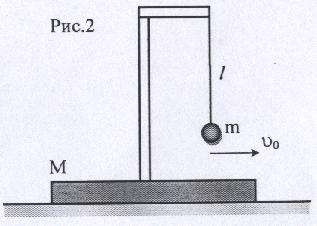
\includegraphics[width = 0.9 \textwidth]{PlatformWithOscillator.png}
\end{minipage}
\begin{ans}
$h= \frac{v_0^2 M}{2g(m+M)}$, $v_2 = 2mv_0/(m+M)$, $T=m(g+v_0^2/l)$
\end{ans}
\end{ex}